\documentclass{beamer}

\usepackage{subfigure}
\usepackage{graphicx}
\usepackage{sidecap}
\usepackage{caption}
%\usepackage{subcaption}
\captionsetup{compatibility=false}
\usepackage{appendixnumberbeamer}
\usepackage{amsmath}
% --
\usepackage{multirow}
\usepackage{xcolor}
\usepackage{setspace}
\usepackage{hyperref}
\usepackage{anyfontsize}

\beamertemplatenavigationsymbolsempty
\setbeamertemplate{footline}

\newenvironment{itemise} {\begin{itemize} \setlength{\itemsep}{0.2cm}} {\end{itemize}}
\usepackage[labelformat=empty]{caption}
\setbeamertemplate{sections/subsections in toc}[square]

%% COLORS
\definecolor{Gray}{gray}{0.9}
\definecolor{dblue}{rgb}{0.132,0.1,0.27}
\definecolor{mint}{cmyk}{1.0, 0.2, 0.6, 0.05}
\definecolor{ant}{cmyk}{0.5, 0.1, 0.0, 0.45}
\definecolor{lgray}{cmyk}{0.12, 0.0, 0.0, 0.17}
\definecolor{lred}{cmyk}{0.0, 0.9, 0.7, 0.0}


\usepackage{etoolbox}% http://ctan.org/pkg/etoolbox 
\usepackage{booktabs}

\newenvironment{literatur}{%
  \parskip2pt \parindent0pt \raggedright
  \def\lititem{\hangindent=0.5cm \hangafter1}}{%
  \par\ignorespaces}

\newcommand{\tb}[1]{{\color{blue}{\textbf{#1}}}}
\newcommand{\tm}[1]{{\color{mint}{\textbf{#1}}}}
\newcommand{\tr}[1]{{\color{red}{\textbf{#1}}}}
% Ilya: packages

\usepackage{tikz}
\usepackage{lmodern}
\usepackage{enumitem}

% Ilya: my commands

\newenvironment{mytemize}
{\vfill\itemize[nolistsep,itemsep=\fill,label=\color{blue}{$\triangleright$}]}
  {\enditemize}

\newcommand{\hitem}[1]{
  {\color{blue}{$\triangleright$}} 
  {#1} 
  {\hfill}
}

\setlist[itemize]{label= \color{blue}{$\triangleright$}}

\newcommand{\rarr}{$\Rightarrow$\ }

\AtBeginSection{%
\ifshowtoc
\begin{frame}
    \tableofcontents[currentsection, subsectionstyle=show/show/hide]
\end{frame}
\fi
}

%\href{<Ziel>}{<Eingefasster Text>} 

%\logo{\includegraphics[height=0.7cm]{BdFlogo.eps}\hspace{300pt}\vspace{-5pt}}
%\logo{\includegraphics[height=0.8cm]{BdFlogo.eps}}
%\logo{\pgfputat{\pgfxy(-6.2,-0.5)}{\pgfbox[center,base]{\includegraphics[height=0.8cm]{BdFlogo.eps}}}}

%------------------------------------------------------------------------------------
% TITLE
%------------------------------------------------------------------------------------
\title[PSME]{Macroeconomics\\ Lecture 6 -- Labor \& Intro to Real Business Cycles }
\author[I. Eryzhenskiy]{Ilya Eryzhenskiy}
\institute[BdF]{PSME Panth\'{e}on-Sorbonne Master in Economics}
\date[PSME macro]{Fall 2023}

\begin{document}

\begin{frame}
   \maketitle 
\end{frame}

\section{Labor Choice}

\begin{frame}{Labor: extensive vs. intensive margin}
    \begin{mytemize}
        \item Extensive margin: do I work at all?
            \begin{mytemize}
                \item Not always a choice: voluntary vs. involuntary unemployment
                \item No theory for this in the course
            \end{mytemize}
        \item Intensive margin: how much do I work?
        \begin{mytemize}
                \item An easier question for neoclassical economics
                \item \tb{Leisure} is a good \rarr Labor $=$ Total time $-$ Leisure
            \end{mytemize}
    \end{mytemize}
\end{frame}

\begin{frame}{Consumption-leisure choice}
  Consider one-period problem of an agent that can work for a total length of time equal to 1 (normalization of work hours \rarr $L$ as \textbf{share} of time devoted to work). She cares for consumption $C$ and leisure time $1-L$:
  \begin{equation*}
	U(\underset{+}{C}, \underset{+}{1-L}) \quad \text{or, equivalently,} \quad U(\underset{+}{C}, \underset{-}{L})
  \end{equation*} 
%  Examples of utility function:  \\
%  $\ln C + \alpha \ln(1-N)$ \\ $\ln C - \alpha/(1+\chi) L^{1+\chi}$ -- in this case, $\chi$ is the inverse of Frisch  elasticity of labor supply -- labor supply under fixed marginal utility of income.
  \vfill 
  Budget constraint:
  \begin{align*}
	P C \leq  W L &\Leftrightarrow C \leq w L \\
		&\Leftrightarrow C + w (1-L) \leq w \quad \text{(consumption vs. leisure)}
  \end{align*} 
  Wage as \textbf{opportunity cost}, or price, of leisure
  

\end{frame}

\begin{frame}{Consumption-leisure choice: graphs, solution}
\end{frame}

\begin{frame}{Consumption and leisure with 2 periods: Lucas-Rapping effect}
  Now consider a 2-period problem with both consumption and leisure. We will assume a specific form of utility function to simplify analysis:
  \begin{align*}
	\max_{C_1, C_2, L_1, L_2}  \{\ln C_1 - \gamma \sigma/(1&+\sigma) L_1^{(1+\sigma)/\sigma}  \\
	&+ \beta(\ln C_2 - \gamma \sigma/(1+\sigma) L_2^{(1+\sigma)/\sigma})\} \\
	\text{s.t.} \quad C_1 + C_2/(1+r) &= w_1 L_1 + w_2 L_2 / (1+r)
  \end{align*}
  
\end{frame}
\begin{frame}{Consumption and leisure with 2 periods: solution}
\end{frame}

\begin{frame}{Lucas-Rapping effect}
  An intertemporal dimension of labor supply through consumption-saving decisions:
  \begin{mytemize}
  \item It is the \textbf{change in time} and not \textbf{average level} of wage that affects labor supply
  \item In periods with temporary wage increases household works more, makes savings, then works less after wage decrease
  \end{mytemize}
\end{frame}
%---FRAME------------------------------------------------------------------------------
\section{Lucas Critique}

\begin{frame}{Lucas critique}

\begin{mytemize}
\small
\item Big "Keynesian macroeconometric models" group  led by Kennedy's Council of Economic Advisers
  \begin{mytemize}
	\item Solow, Tobin, Samuelson
  \end{mytemize}
\item Application of IS-LM (IS-TR), Mundell-Flemming (Is-TR-IFM), AD-AS models to the data. Models represented as system of linear equations and estimated by least-squares methods:
\end{mytemize}
\begin{figure}[h!]
%\caption{Figure. Net}
	\subfigure{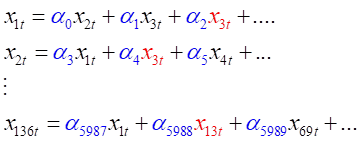
\includegraphics[trim=0 0 0 0,clip,width=0.6\textwidth]{FIGURES/9_LCritiqueMatrix}
	}      
	%} 		
%	\label{fig:GPD} 
	%[trim=left bottom right top
\end{figure}

\begin{mytemize}
\small
\item \tb{R. Lucas' idea (1976)}: The alphas (e.g. marginal propensity to consume) are \tr{endogenous} with respect to government policy
\end{mytemize}

\end{frame}

\begin{frame}{Lucas critique II}
  Lucas's critique has received a huge response from macro theorists. \\
  \vfill 
  Instead of modelling \tr{accounting relationships} such as $Y = C + I + G + PCA$\dots
  \vfill
  \dots starting to model \tb{rational agents' behaviour}
  \vfill
  Two essential elements:
  \begin{mynumerate}
	\item All agents \tb{optimize} some objective function. Utility for households, profit for firms.
	\item \tb{Rational expectations}: agents know the structure of the economy (the model), errors are possible, but not \textbf{systematic} 
  \end{mynumerate}
  \vfill 
  End of microeconomics vs. macroeconomics divide, everything is \tb{micro-founded}.

\end{frame}
%---FRAME------------------------------------------------------------------------------
%\section{Overview}
\begin{frame}{Lucas critique: examples}
  \small
  Consider households' reaction to a positive government spending shock:
  \begin{mytemize}
  \item If \tb{temporary}, need to know how many years it will last: consumption response is not same if GDP (and incomes) boosted for 1 year and of boosted for 5 years 
  \item If \tb{permanent}, government debt accumulation \rarr consumers need to know what is the debt reduction strategy of government
	\begin{mytemize}
	\item If taxes will be raised in the future, households need to increase savings now to prepare for decrease of income \rarr \textbf{smaller marginal propensity to consume today}
	\item If central bank not independent and finances government deficit with additional money supply, inflation expected to rise \rarr better buy things now while prices low \rarr \textbf{higher marginal propensity to consume today}
	\end{mytemize}
  \end{mytemize}
  \vfill
  Households' consumption reaction interacts with \tb{labor supply} \rarr under sticky wages, wage and price setting (and AS) influenced by factors listed above.
\end{frame}
\section{Introduction to business cycles}
\begin{frame}{What are business cycles?}

  Historically, Smith, Marx, Kondratiev and others thought of cycles literally --- economic indicators following sine waves
  \vfill
  Famous example (not macro) --- pork cycles:
  \vfill
\begin{center}
\begin{figure}[h!]
	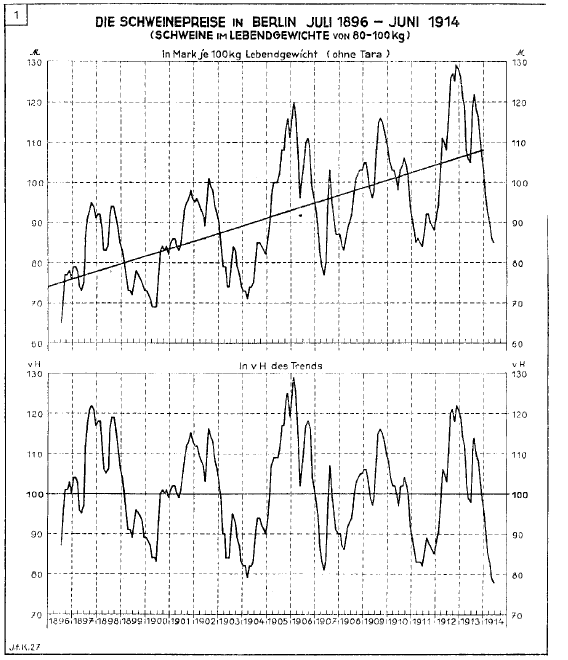
\includegraphics[clip,width=0.4\textwidth]{FIGURES/1_PorkCycle_a}
\caption{Pork prices in Berlin, July 1896 - June 1914}
%	\label{fig:GPD} 
\end{figure}
%\vspace{-2mm}
%\begin{minipage}{1.0\columnwidth}
%\tiny	
%%\textbf{Note.} .\\
% \textbf{Source.} von Hanau, Arthur (1928) 'Die Prognose der Schweinpreise', in: \emph{Vierteljahreshefte zur Konjunkturforschung}, Sonderheft 7. Berlin: Institut f\"{u}r Konjunkturforschung, \href{https://www.diw.de/documents/dokumentenarchiv/17/diw_01.c.43353.de/viertel_1928.pdf}{[Link]}.\\
%\end{minipage}
\end{center}

\end{frame}
%---FRAME------------------------------------------------------------------------------
%---FRAME------------------------------------------------------------------------------
%\begin{frame}{Income and Output}
%
%\begin{mytemize}
%{\footnotesize
%\item \tb{Gross domestic product} (GDP): \emph{Indicator of the goods and services produced within an economy in a year for final use, a nation's economic well-being.}
%}
%\end{mytemize}
%\vspace{-5mm}
%\begin{center}
%\begin{figure}[h!]
%	\subfigure{\includegraphics[clip,width=0.95\textwidth]{../PSME_stata/FIGURES/1_GDP}
%	}      
%%	\label{fig:GPD} 
%\end{figure}
%\vspace{-2mm}
%\begin{minipage}{0.9\columnwidth}
%\tiny	
%%\textbf{Note.} .\\
% \textbf{Source.} Jorda-Schularick-Taylor Macrohistory Database \href{http://www.macrohistory.net/data/}{[Link]} .\\
%\end{minipage}
%\end{center}
%
%\end{frame}
%---FRAME------------------------------------------------------------------------------
%\begin{frame}{Trend vs. cycle}
%
%\begin{mytemize}
%\item Steady trend in \tb{economic growth} (GDP) over time.
%\item Recurring fluctuations of GDP around its trend ($\rightarrow$\tb{business cycle})
%\end{mytemize}
%
%\begin{center}
%\begin{figure}[h!]
%	\subfigure{\includegraphics[clip,width=0.95\textwidth]{../PSME_stata/FIGURES/1_GDPtrendcycle}
%	}      
%%	\label{fig:GPD} 
%\end{figure}
%\vspace{-2mm}
%\begin{minipage}{0.9\columnwidth}
%\tiny	
%\textbf{Note.} Trend-cycle decomposition using a Hodrick-Prescott filter with a smoothing value of 6.25.\\
% \textbf{Source.} Own calculations. Jorda-Schularick-Taylor Macrohistory Database.\\
%\end{minipage}
%\end{center}
%
%\end{frame}
%---FRAME------------------------------------------------------------------------------
\begin{frame}{Towards modern business cycles}

\begin{mytemize}
\item \tb{National Bureau of Economic Research} (NBER), founded 1920, influential group of economists
\item Persuaded that statistical methods make study of economic phenomena (cycles) possible
\item Idea by Arthur Burns \& Wesley Mitchell:
\begin{mytemize}
\item Focus on boom and bust periods $\Leftrightarrow$ peaks and troughs of cycle
\item Identify common patterns for different booms and busts
\end{mytemize}
%\item NBER still influential in macroeconomics. See working papers: \tiny
%  \begin{mytemize}
%  \item \url{https://www.nber.org/programs-projects/programs-working-groups/economic-fluctuations-and-growth?page=1&perPage=50}
%  \end{mytemize}
\end{mytemize}

\end{frame}

\begin{frame}{Burns-Mitchell Diagrams: an example}

\begin{columns}
          \column{0.50\linewidth}
             \centering
             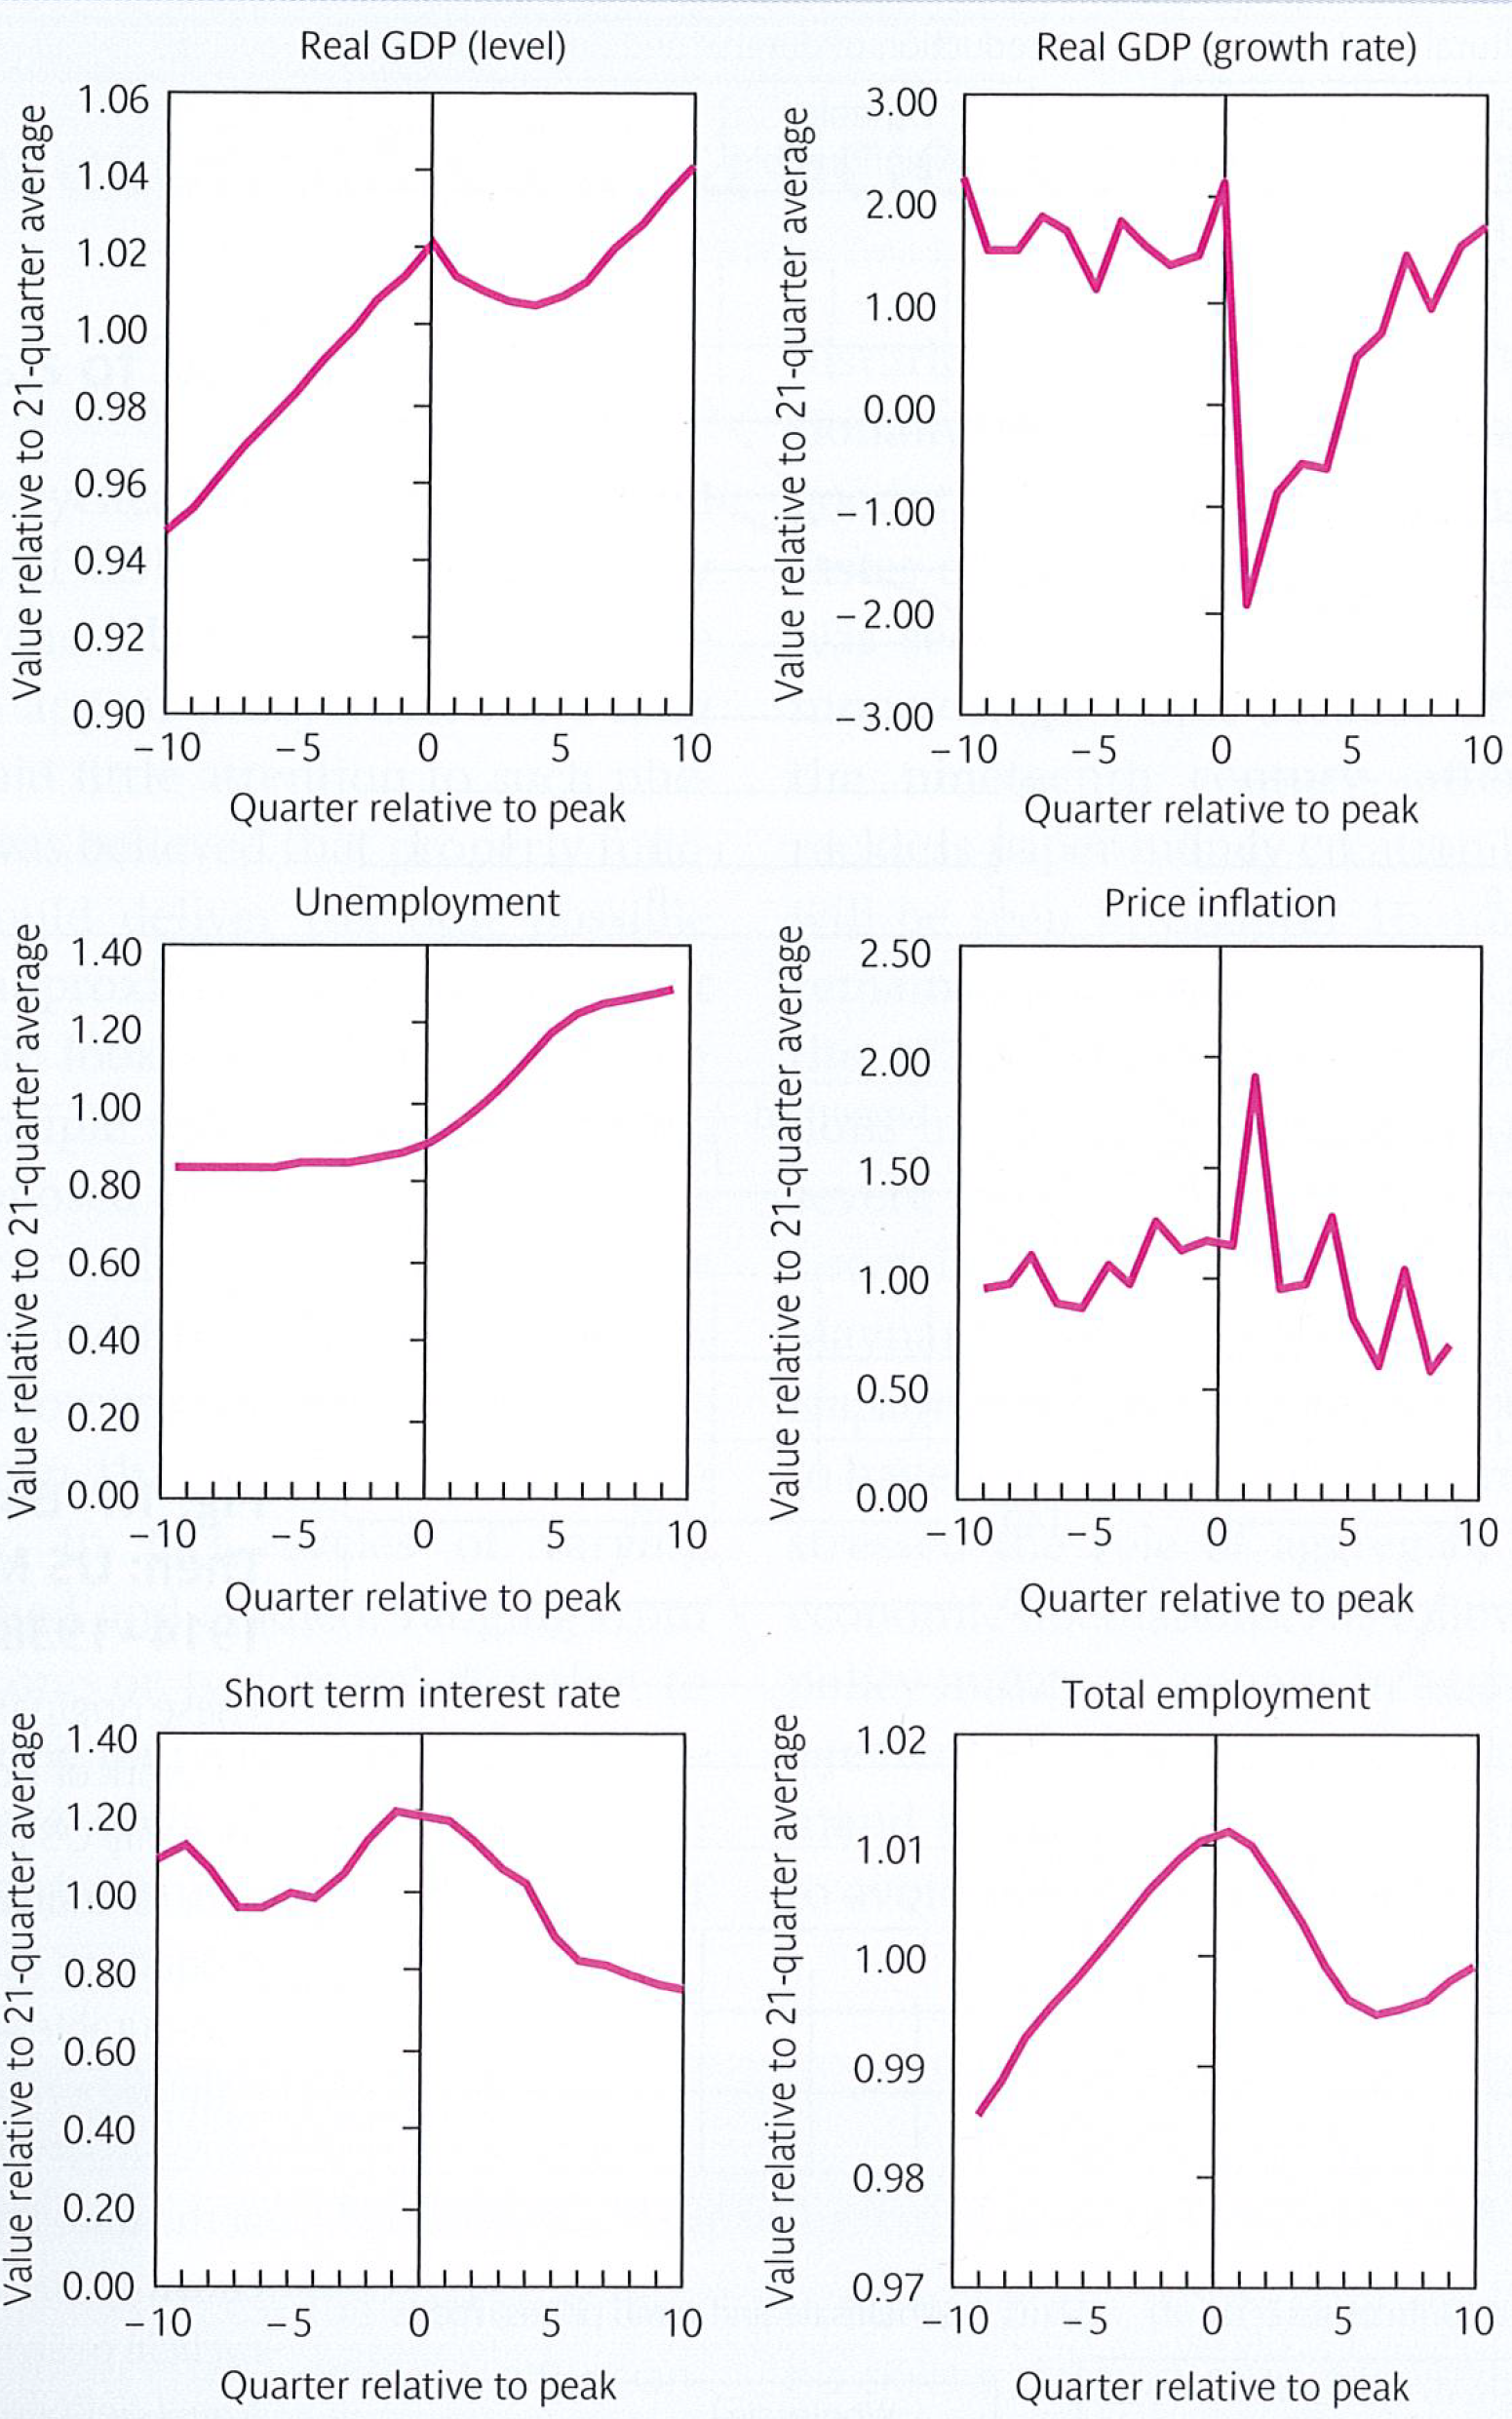
\includegraphics[clip,width=0.8\columnwidth]{FIGURES/1_BurnsMitchell_b}
           \vspace{-2mm}
	\begin{minipage}{1.0\columnwidth}
%	\tiny	
%	\textbf{Note.} The Figure shows the average behaviour of variables around cyclical peaks in eight countries.\\
% 	\textbf{Source.} Burda and Wyplosz (2013), Figure 1.6 (p. 13).\\
	\end{minipage}
	% COLUMN(2)
    \column{0.50\linewidth}
           
\begin{mytemize}
\item peak of GDP = vertical line
\item Unemployment = \tb{countercyclical}
\item Inflation = procyclical (\textbf{\emph{lagging}} the cycle)
\item Short term interest rate, employment = \tb{procyclical}
\end{mytemize}


%	\begin{minipage}{0.9\columnwidth}		
%	\tiny
%	\begin{singlespace*}
%	$^*$ The peak is determined using a procedure proposed by Harding and Pagan (2001) 'Dissecting the Cycle: A Methodological investigation', \emph{Journal of Monetary Economics}, 49(2); see Burda \& Wyplosz Box 1.1 for methodological details.          	
%	\end{singlespace*}
%	\end{minipage}
	
	
\end{columns} 
	       

\end{frame}

\begin{frame}{Recession dating by NBER}
  \centering
             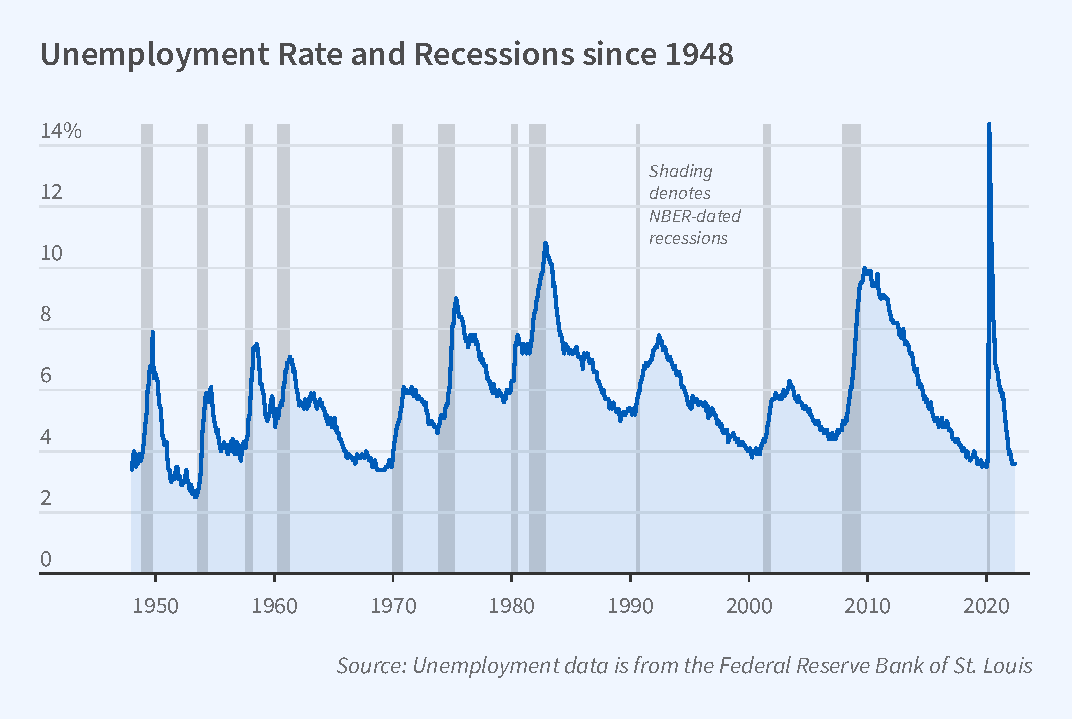
\includegraphics[width=0.9\textwidth]{FIGURES/nber_unemp_aft1948}
\end{frame}


\section{Business Cycles in a Small Open Economy: Data}

\begin{frame}{Canadian Economy: Business-Cycle Statistics}
  Canada -- developed economy, but 2.1 \% of world GDP \rarr ``small'' (compare to China -- 18.4\%; USA -- 24\% -- large open economies). 
  \vfill
  We will seek to explain historical business-cycle patterns: 1946-1985.
  \vfill
\centerline{
\begin{tabular}{|c|c|c|c|}
\hline
Variable ($x_t$)&\multicolumn{3}{|c|}{Moments}\\
\cline{2-4}
&$\sigma_{x_t}$
&corr$(x_t,x_{t-1})$
&corr$(x_t,Y_t)$
\\
\hline
$Y$           &  2.8&  0.61&      1\\
$C$           &  2.5&   0.7&   0.59\\
$I$           &  9.8&  0.31&   0.64\\
$L$           &    2&  0.54&    0.8\\
$\frac{TB}{Y}$&  1.9&  0.66&  -0.13\\
\hline
\end{tabular}}

\centerline{\tiny Source: Mendoza AER, 1991. Annual data. Log-quadratically detrended.}

\end{frame}

\end{document}